\documentclass{article} % use larger type; default would be 10pt
\usepackage[utf8]{inputenc} % set input encoding (not needed with XeLaTeX)
\usepackage{geometry} % to change the page dimensions
\geometry{a4paper} % or letterpaper (US) or a5paper or....
\usepackage{graphicx} % support the \includegraphics command and options
\usepackage{booktabs} % for much better looking tables
\usepackage{paralist} % very flexible & customisable lists (eg. enumerate/itemize, etc.)
\usepackage{verbatim} % adds environment for commenting out blocks of text & for better verbatim
\usepackage{subfig} % make it possible to include more than one captioned figure/table in a single float
\usepackage{fancyhdr} % This should be set AFTER setting up the page geometry
\usepackage{newtxtext}
\usepackage{graphicx}
\usepackage{float}
% Define header and footer styles
\fancypagestyle{myfancy}{
  \fancyhf{} % Clear default header and footer
  \fancyhead{} % Clear default header
  \fancyfoot[C]{\thepage} % Set centered page number in footer
  \renewcommand{\headrulewidth}{0pt} % Remove header line
  \renewcommand{\footrulewidth}{0.4pt} % Add footer line
  \fancyhead[C]{\rule{\linewidth}{0.4pt}} % Add line at top of page for header
}

% Apply the new style
\pagestyle{myfancy}

\title{Dynamic Relationships in Environmental and Energy Data: A Time Series Approach}
\author{CHITA Ionut-Cristian, COJOCARITA Cristian}
\date{}
\begin{document}
\maketitle
\tableofcontents

\section{Introduction}
It is essential to comprehend how temperature, energy use, and air quality interact in order to combat global warming and enhance environmental health. In order to examine these factors this study focuses on three important time series datasets. We investigate daily temperature, air quality (PM2.5 levels), and thermal energy balance in an effort to find trends and connections that illustrate how human activity affects the environment.

\subsection{Balance of Thermal Energy by Component Elements}
\begin{itemize}
    \item \textbf{Definition:} Tracks the flow of thermal energy through various stages, including primary production, imports, exports, and consumption by sectors like industry, transport, and households. It also accounts for losses and statistical differences.
    \item \textbf{Periodicity:} Semi-annually, from 1992 to 2022
    \item \textbf{Measurement Unit:} Terajoules
    \item \textbf{Source:} Tempo Online: \textbf{IND111A}
\end{itemize}

\subsubsection*{Contextualization:}
For the purpose of creating comprehensive energy policies and plans that aim for sustainability, it is essential to comprehend the balance of thermal energy by its constituent parts. This information gives us an understanding of the efficiency and environmental effect of energy consumption by allowing us to examine how energy is generated, used, and lost across many sectors. The significance of this analysis is emphasized by a number of important research and reports.

First off, the Reveiu et al. (2015) study emphasizes how important it is to incorporate consumer behavior into techno-economic energy models. The study shows that conventional models, which solely take into account technological and economic aspects, frequently fall short of accurately capturing the real dynamics of energy usage. These models can anticipate energy consumption and spot potential for efficiency gains more precisely by include behavioral data. This method, which takes into account both technological and behavioral factors that affect energy usage and losses, is especially pertinent to comprehending the thermal energy balance [1].

Furthermore, Gherhes and Fărcas's study from 2021 on sustainable behavior among Romanian students offers a more comprehensive explanation of the significance of monitoring thermal energy balance. According to their research, behavior modifications can result in considerable energy savings and residential energy usage is a key contributor to total energy use. Having a thorough understanding of the precise thermal energy flow, including the locations of losses, may aid in the creation of focused interventions that cut waste and boost productivity. Promoting energy-efficient equipment and practices, for example, may greatly reduce thermal energy consumption and losses in homes [2].

In addition, a thorough assessment of techno-economic models is included in the paper of Timmerman et al. (2014), which classifies several models that aid in the evaluation of energy systems. They contend that these models may be made much more accurate by incorporating both current energy flow data and long-term estimates. The requirement for comprehensive thermal energy balance data is supported by this method, which may help guide current and future energy policy [3].

The balance of thermal energy by component elements serves as a tactical instrument for policymakers. We can better address the issues around energy sustainability if we have a greater understanding of the production, transmission, and consumption of energy across many industries. Developing policies that lower greenhouse gas emissions, increase energy efficiency, and encourage the use of renewable energy sources requires a comprehensive approach.

\subsubsection*{References:}

\begin{enumerate}
    \item Reveiu, A., Smeureanu, I., Dardala, M., Kanala, R. (2015). Modelling Domestic Lighting Energy Consumption in Romania by Integrating Consumers Behavior. \textit{Procedia Computer Science}, 52, 812-818. 
    \item Gherhes, V., Fărcas, M. A. (2021). Sustainable Behavior among Romanian Students: A Perspective on Electricity Consumption in Households. \textit{Sustainability}, 13(9357), 1-17.
    \item Timmerman, J., Vandevelde, L., Van Eetvelde, G. (2014). Towards low carbon business park energy systems: Classification of techno-economic energy models. \textit{Energy}, 75, 68-80.
\end{enumerate}

\subsection{Popesti-Leordeni AQI PM2.5 Daily}
\begin{itemize}
    \item \textbf{Definition:} The Air Quality Index (AQI) for PM2.5 represents the daily average concentration of particulate matter smaller than 2.5 micrometers in diameter. This index indicates air quality and potential health effects.
    \item \textbf{Periodicity:} Daily
    \item \textbf{Measurement Unit:} Micrograms per cubic meter (\textbf{µg/m³})
    \item \textbf{Source:} AQICN Popesti-Leordeni: \textbf{https://aqicn.org/station/@109861}
\end{itemize}

\subsubsection*{Contextualization:}
An important environmental health indicator is air quality, specifically the amount of fine particulate matter (PM2.5) in the atmosphere. Tracking PM2.5 levels helps determine the efficacy of air quality-improving programs as well as changes in air pollution. The significance of monitoring PM2.5 concentrations and their effects on the environment and public health is highlighted in a number of research and reports.

A thorough inventory of Romania's principal air pollutants and air quality was carried out by Năstase et al. (2018), who also noted the serious concerns that air pollution poses to the environment, the economy, food security, and public health. The report highlights that the production and use of fossil fuels is the primary source of most pollutants, including PM2.5. Romania's consumption of fossil fuels has decreased during the last ten years, mostly as a result of EU rules that promote the use of renewable energy sources. PM emissions have decreased as a result of this change, but ongoing observation is necessary to assess the long-term efficacy of these efforts.[4]

A research by Burghele et al. (2021) on interior air quality in energy-efficient buildings in Romania emphasizes the intricacies of air pollution, which further supports the need for air quality monitoring. According to the study, if energy saving measures in buildings are not adequately maintained, they may unintentionally result in poor indoor air quality. This is especially important for PM2.5 since poorly ventilated, highly insulated buildings can trap pollutants within, increasing the danger to health.[5]

In addition, because PM2.5 may enter the bloodstream and pierce deeply into the lungs, the World Health Organization (WHO) lists it as one of the most dangerous air pollutants. Long-term exposure to PM2.5 has been associated with higher death rates as well as cardiovascular and respiratory disorders. Thus, monitoring daily PM2.5 levels is essential for public health surveillance and for putting appropriate actions in place to lessen its effects.[6]

In conclusion, this information supports strategies to lower emissions and exposure to dangerous pollutants, as well as aids in the identification of pollution sources and the assessment of the efficacy of air quality legislation.

\subsubsection*{References:}
\begin{enumerate}
    \item Năstase, G., Șerban, A., Năstase, A.F., Dragomir, G., Brezeanu, A.I. (2018). Air quality, primary air pollutants and ambient concentrations inventory for Romania. Atmospheric Environment.
    \item Burghele, B.D., et al. (2021). Comprehensive survey on radon mitigation and indoor air quality in energy-efficient buildings from Romania. Science of the Total Environment, 751, 141858.
    \item World Health Organization (WHO). (2018). Air quality guidelines for particulate matter.
\end{enumerate}
These sources offer a thorough grasp of the significance of controlling and monitoring air quality, especially PM2.5 levels, in order to protect the environment and human health.

\subsection{Popesti-Leordeni Temperature Daily}
\begin{itemize}
    \item \textbf{Definition:} The daily average temperature measurement records the atmospheric temperature at a specific location, providing insights into daily climatic conditions.
    \item \textbf{Periodicity:} Daily
    \item \textbf{Measurement Unit:} Celsius
    \item \textbf{Source:} AQICN Popesti-Leordeni \textbf{https://aqicn.org/station/@109861}
\end{itemize}

\subsubsection*{Contextualization:}
It is essential to monitor daily temperature data in order to comprehend climatic variability and recognize long-term patterns. Numerous research works have emphasized the need of temperature monitoring in evaluating the effects of climate change, particularly in areas such as Romania where notable warming has been seen in recent years.

Noteworthy trends in annual air temperature were found in a comprehensive research on climate changes in Romania by Marin et al. (2014). Other noteworthy trends in climate variables included precipitation, sunlight hours, and cloud cover. The study employed the Mann-Kendall trend test and Kendall-Theil technique, utilizing data from all accessible meteorological stations in Romania from 1961 to 2013, to identify statistically significant increases in air temperature throughout the nation. The results show a general trend toward warming, with the air temperature showing the most shifts—it rose at every location under analysis. The region is being impacted by greater global warming tendencies, which are highlighted by this steady increase in temperature.[7]

In a similar vein, Birsan et al. (2019) employed the Mann-Kendall test on gridded daily data from the ROCADA dataset covering the years 1961 to 2013 to examine variations in yearly temperature extremes over Romania. The analysis discovered rising trends in warm-related extremes and declining trends in cold-related indicators, such as the quantity of frost days. The asymmetric patterns of daylight vs nocturnal warming are highlighted by these shifts, which are especially noticeable in lowland areas. The study highlights the significance of geographic factors in climate variability by indicating that the observed warming trends are more strongly correlated with altitude than latitude.[8]

These results are further supported by Piticar and Ristoiu's (2012) study on the evolution of air temperature in Northeastern Romania. Their examination of data spanning 50 years (1961–2010) revealed notable upward trends in air temperature, especially in the summer months of June, July, and August. The robustness of these warming patterns was verified by the use of many statistical tests, such as Sen's slope estimation and the Mann-Kendall test. The height of the weather stations has an impact on temperature trends, with lower elevation stations exhibiting more dramatic warming, according to the study's hierarchical cluster analysis.[9]

All of these studies emphasize how important it is to track and examine daily temperature data in order to comprehend the dynamics of the local climate. Romania's steady warming tendencies are consistent with patterns of climate change worldwide, which offers crucial information for creating mitigation and adaptation plans.

\subsubsection*{References:}
\begin{enumerate}
    \item Marin, L., Birsan, M.V., Bojariu, R., Dumitrescu, A., Micu, D.M., Manea, A. (2014). An overview of annual climatic changes in Romania: trends in air temperature, precipitation, sunshine hours, cloud cover, relative humidity and wind speed during the 1961–2013 period. Carpathian Journal of Earth and Environmental Sciences, 9(4), 253-258.
    \item Birsan, M.V., Micu, D.M., Niță, I.A., Mateescu, E., Szép, R., Keresztesi, Á. (2019). Spatio-temporal changes in annual temperature extremes over Romania (1961–2013). Romanian Journal of Physics, 64, 816
    \item Piticar, A., Ristoiu, D. (2012). Analysis of air temperature evolution in northeastern Romania and evidence of warming trend. Carpathian Journal of Earth and Environmental Sciences, 7(4), 97-106
\end{enumerate}

\section{Application 1: ARMA/ARIMA Models in EViews}
\subsection{Unit Root Tests:}

\begin{figure}[H]
    \centering
    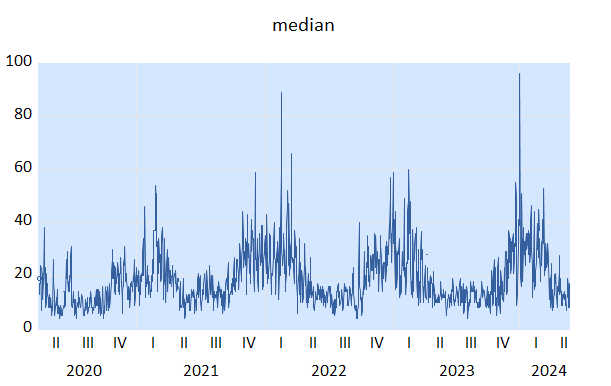
\includegraphics[width=10cm]{images/image10.png}
    \caption{Air Quality Index in Bucharest (Popesti-Leordeni)}
\end{figure}

The AQI fluctuates significantly between 2020 and 2024, as seen in Figure 1, with values ranging from 0 to over 100. The spikes show times when the quality of the air was low, perhaps as a result of things like increased industrial activity or vehicle emissions.

\begin{figure}[H]
    \centering
    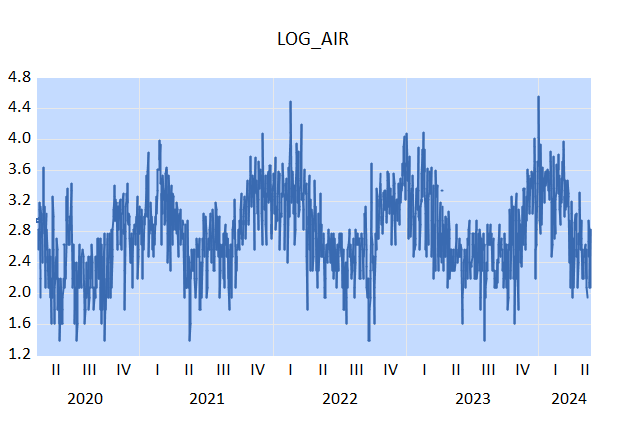
\includegraphics[width=10cm]{images/image20.png}
    \caption{Log Transformation of Air Quality Index}
\end{figure}

The AQI's log transformation is displayed in Figure 2, which reduces higher values and increases lower ones to stabilize the variance. Though variations persist, this change makes underlying patterns more evident.

\begin{figure}[H]
    \centering
    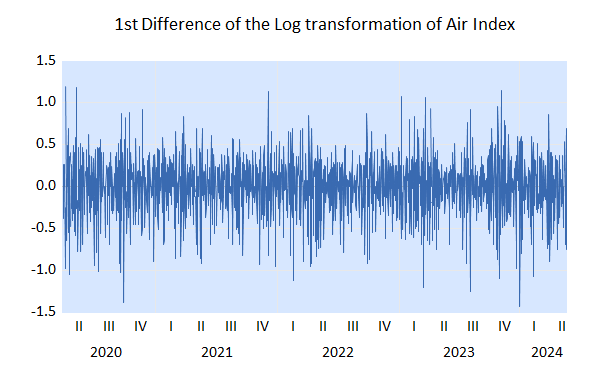
\includegraphics[width=10cm]{images/image36.png}
    \caption{1st Difference of the Log Transformation of Air Index}
\end{figure}

The initial difference of the log-transformed AQI, which eliminates trends and increases series stationaryity, is shown in Figure 3. The values show more consistent fluctuations over time and a more steady mean as they oscillate about zero.

\begin{itemize}
    \item Original Series: High variability and significant spikes in AQI.
    \item Log Transformation: Stabilizes variance and clarifies patterns.
    \item First Difference of Log Transformation: Stabilizes mean, suggesting closer stationarity. Further tests are needed to confirm.
\end{itemize}

These transformations help prepare the AQI data for accurate time series analysis and forecasting.

\begin{figure}[H]
    \centering
    \begin{minipage}{0.5\linewidth}
        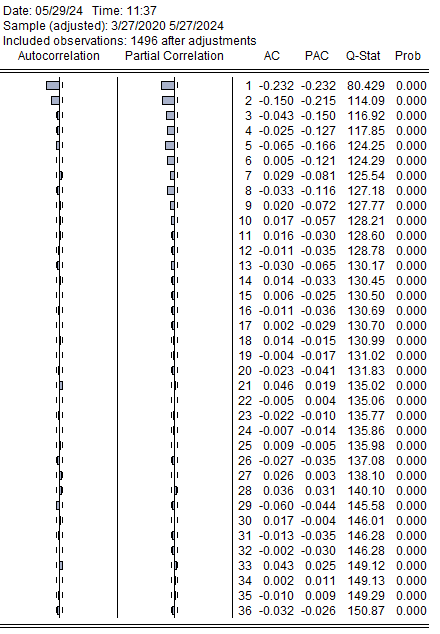
\includegraphics[width=\linewidth]{images/image9.png}
        \caption{SACF and SPACF of the transformed Time Series}
    \end{minipage}%
    \begin{minipage}{0.5\linewidth}
        \subsubsection*{Correlogram of D\_LOG\_AIR}
        \begin{itemize}
            \item \textbf{ACF:} Significant spikes at initial lags, indicating autocorrelation.
            \item \textbf{PACF:} Significant spikes at initial lags, suggesting AR and/or MA components.
            \item \textbf{Interpretation:} The ACF and PACF show significant values, indicating the presence of AR and/or MA components in the data.
        \end{itemize}
    \end{minipage}
    \caption{ProbADF calculated for AIR Index in Popesti-Leordeni}
\end{figure}

We can observe that the PP test, the ADF test, and the KPSS test all point to a stationary time series from the table that combines the p-values of the ADF, Philips-Peron, and KPSS tests. Therefore, we will choose to proceed with an integration order of d = 1. It is implied that {log AIR}t ~ ARIMA(p, 1, q) for our consideration of ARIMA models.

\begin{figure}[H]
    \centering
    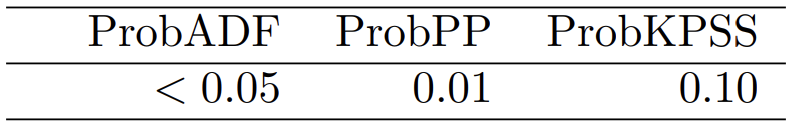
\includegraphics[width=10cm]{images/image15.png}
\end{figure}

We can find below a quick reminder for the hypothesis related to the ADF and the PP tests4 for a given time series: 

\begin{figure}[H]
    \centering
    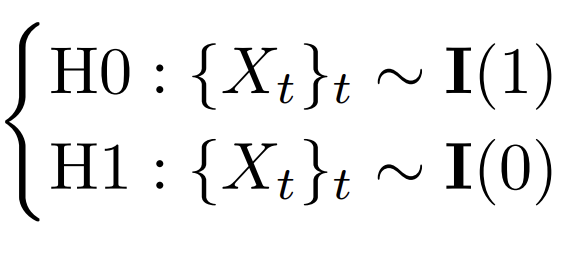
\includegraphics[width=5cm]{images/image24.png}
\end{figure}

\begin{figure}[H]
    \centering
    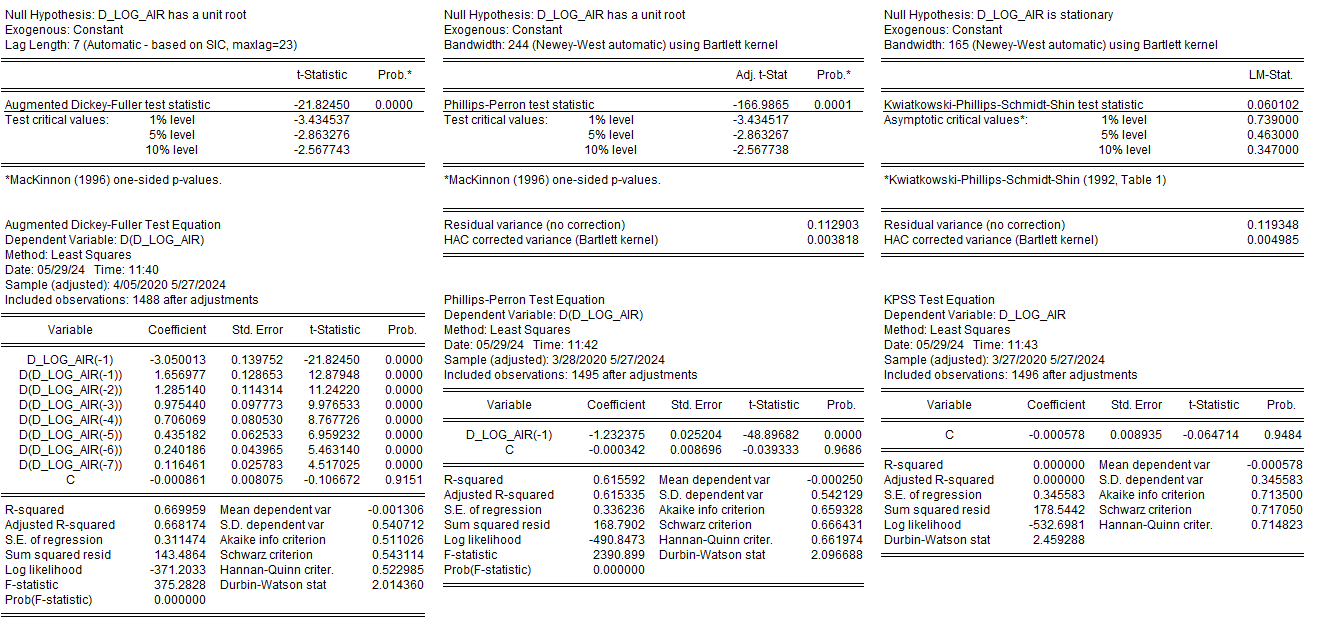
\includegraphics[width=\linewidth]{images/image16.png}
    \caption{ProbADF,ProbPP,ProbKPSS computed for Log Air Index Difference of Transformation}
\end{figure}

\begin{figure}[H]
    \centering
    \begin{minipage}{0.5\linewidth}
        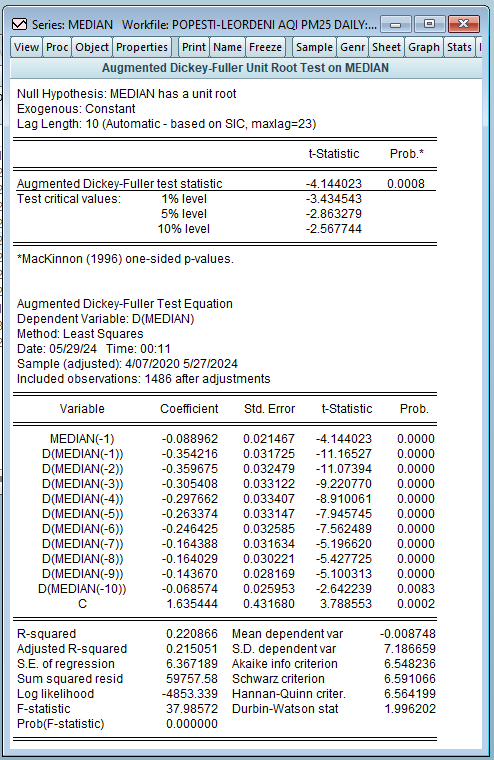
\includegraphics[width=\linewidth]{images/image12.png}
    \end{minipage}%
    \begin{minipage}{0.5\linewidth}
        \begin{enumerate}
            \item \textbf{Stationarity:} The ADF test results indicate that the AIR index (median) is stationary after differencing. This is evidenced by the ADF test statistic being lower than the critical values and the p-value being below 0.05.
            \item \textbf{Significant Lags:} The test equation shows that several lagged differences of the median AQI are significant, with p-values less than 0.05, indicating that past values significantly affect the current differenced value.
            \item \textbf{Model Fit:} The R-squared value of 0.220866 suggests that approximately 22.1\% of the variance in the differenced series is explained by the model. While this indicates some explanatory power, there is still substantial unexplained variance.
        \end{enumerate}
    \end{minipage}
\end{figure}

\subsection{Box-Jenkins methodology and model validity}
Using the auto.arima function, the best model is indeed confirming our intuition. Based on AIC, BIC, and LL criterions the best model is ARIMA(1, 1, 1) with drift. Since the program may not be correct every time, we will keep using ARIMA(1, 1, 0) with drift, based on our intuitions, and compare the two models. First, looking at the criteria, ARIMA(1, 1, 1) is indeed slightly better. 

From the estimation output, we obtain the following model for ARIMA(1, 1, 1):

\begin{verbatim}
LOG_AIR = 2.79014008875 + 0.500059151561*D(LOG_AIR) + 
[AR(1)=0.769568358748,MA(1)=0.999999220557,UNCOND,ESTSMPL="3/27/2020 5/27/2024"]
\end{verbatim}

For ARIMA(1, 1, 0):

\begin{verbatim}
LOG_AIR = 2.78935651999 + 0.500546810534*D(LOG_AIR) + [AR(1)=0.899799843248,UNCOND]
\end{verbatim}

We must now verify the two models' validity because, as the ACF functions in Figure 8 and 9 show, the autocorrelation is negligible. As a result, the standard errors are accurately computed, suggesting that we may easily verify if the coefficients are true.

\begin{figure}[H]
    \centering
    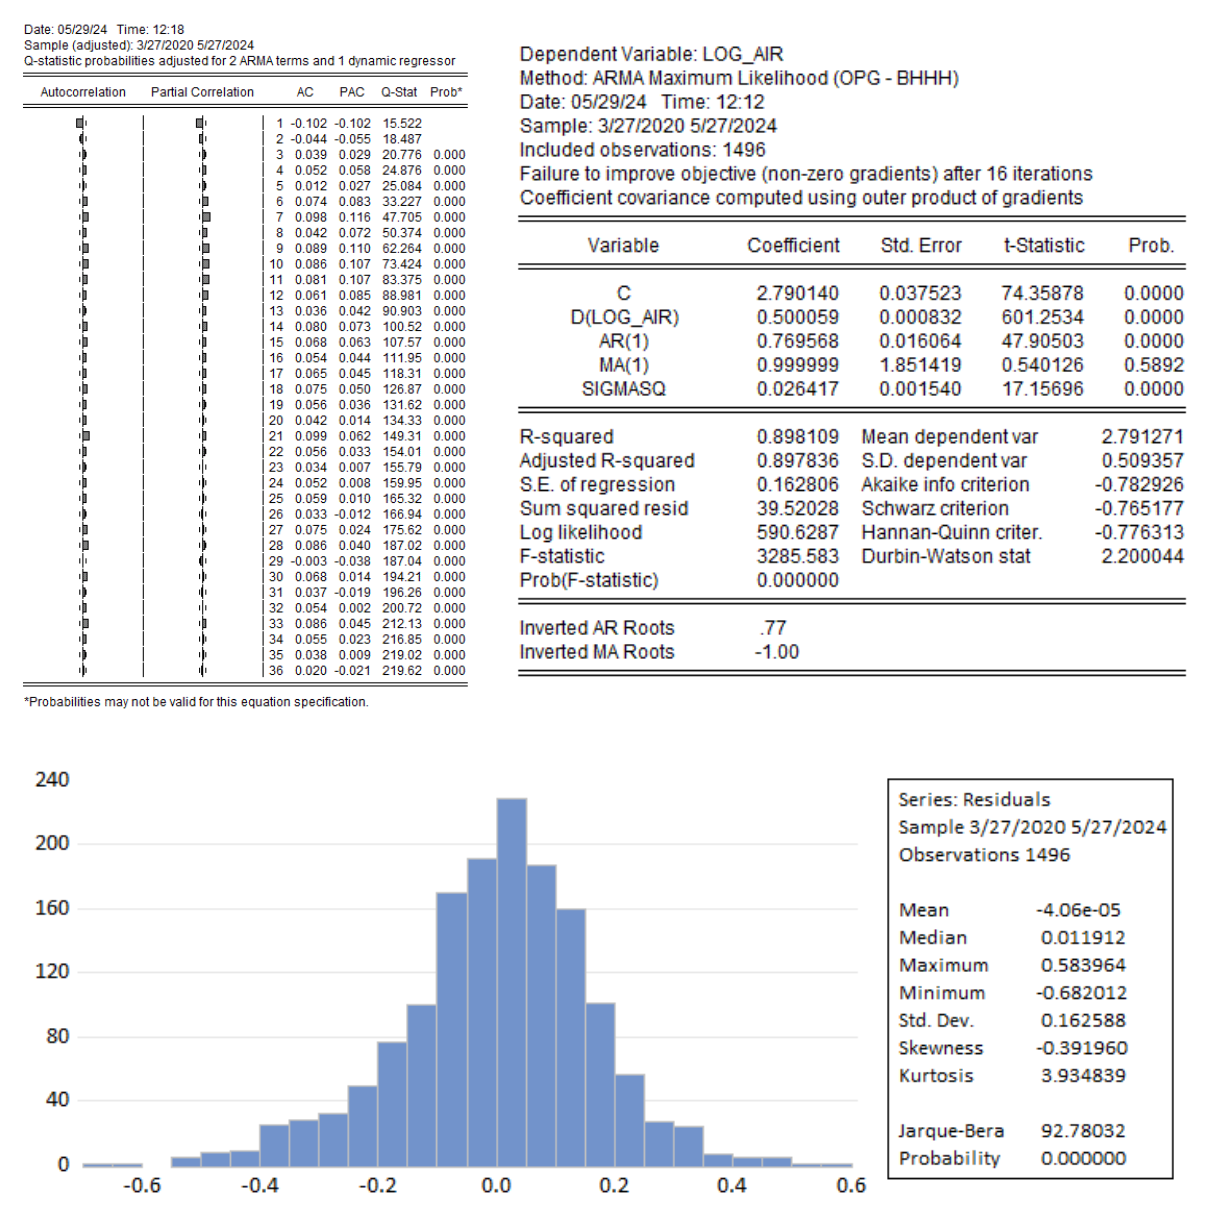
\includegraphics[width=10cm]{images/image17.png}
    \caption{Residuals from ARIMA(1,1,1)}
\end{figure}

\begin{figure}[H]
    \centering
    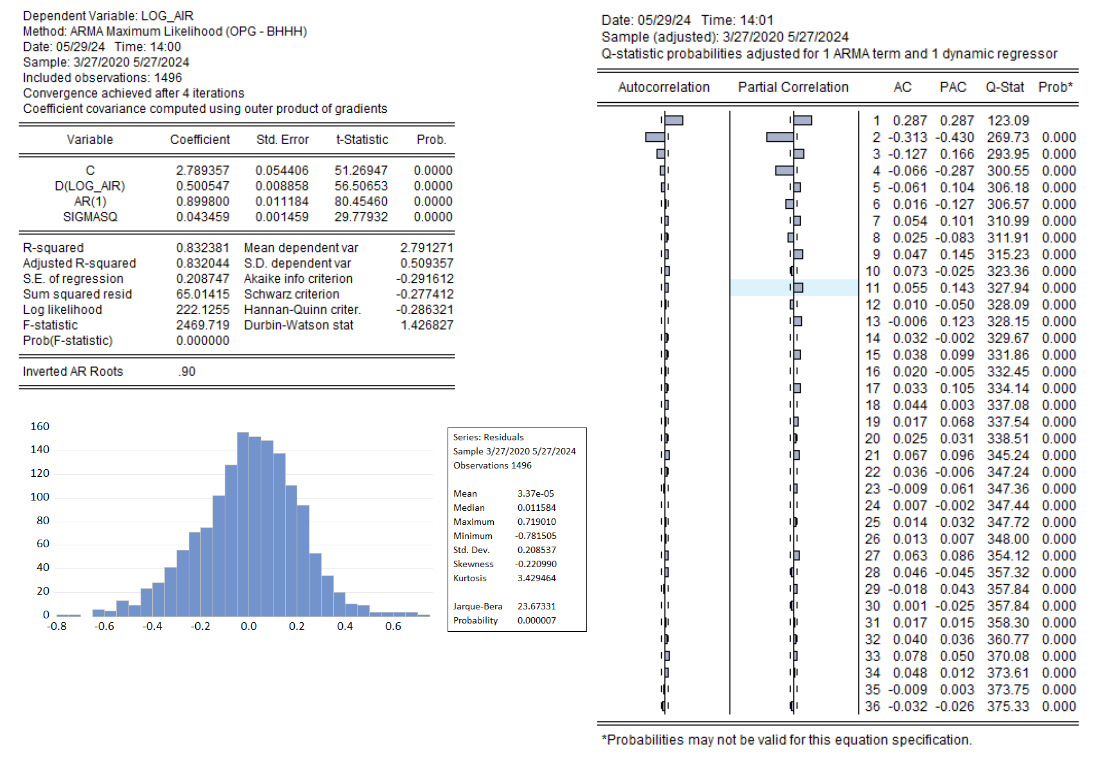
\includegraphics[width=10cm]{images/image40.png}
    \caption{Residuals from ARIMA(1,1,0)}
\end{figure}

\subsubsection*{Forecast Output Analysis:}

\begin{figure}[H]
    \centering
    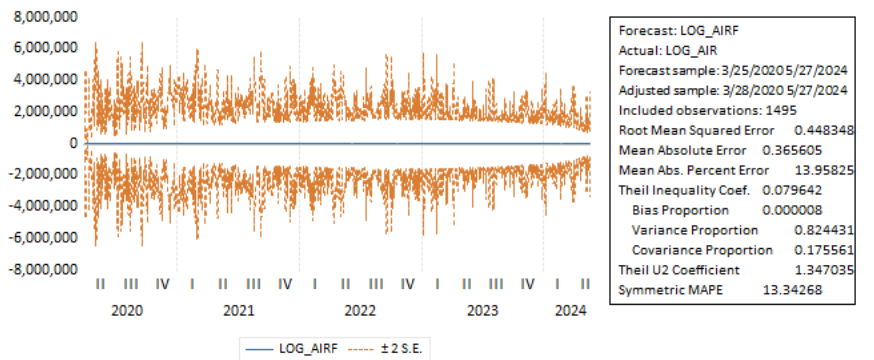
\includegraphics[width=10cm]{images/image41.png}
\end{figure}

\begin{figure}[H]
    \centering
    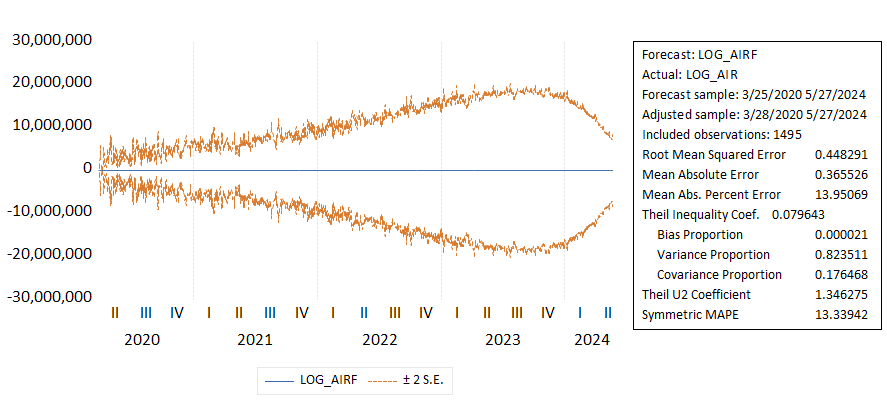
\includegraphics[width=10cm]{images/image26.png}
\end{figure}

\begin{figure}[H]
    \centering
    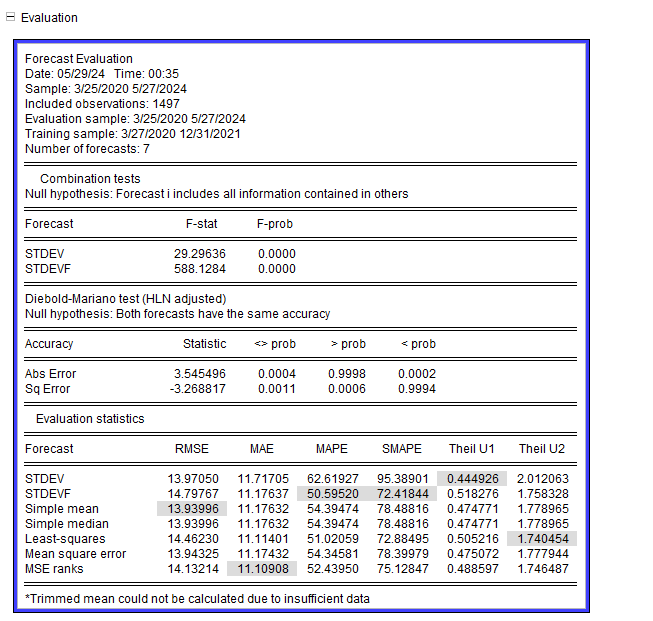
\includegraphics[width=10cm]{images/image38.png}
\end{figure}

\subsubsection*{Forecast Evaluation Table}
\begin{itemize}
    \item The combination tests indicate that each forecast model (STDEV, STDEVF) contains unique information not captured by the other, as both F-statistics are significant (p < 0.05).
    \item The significant p-values (< 0.05) for both absolute and squared errors indicate that there is a statistically significant difference in the accuracy of the forecasts.
    \item Best Performing Model: The Simple Mean model appears to perform best overall based on RMSE and MAE.
    \item STDEV Models: While the STDEV and STDEVF models capture more extreme fluctuations, they tend to have higher errors and variance.
    \item Overall Fit: The forecasts provide a reasonable approximation of the actual values, but the choice of model may depend on the specific error metrics prioritized (e.g., RMSE vs. MAPE).
\end{itemize}

\begin{figure}[H]
    \centering
    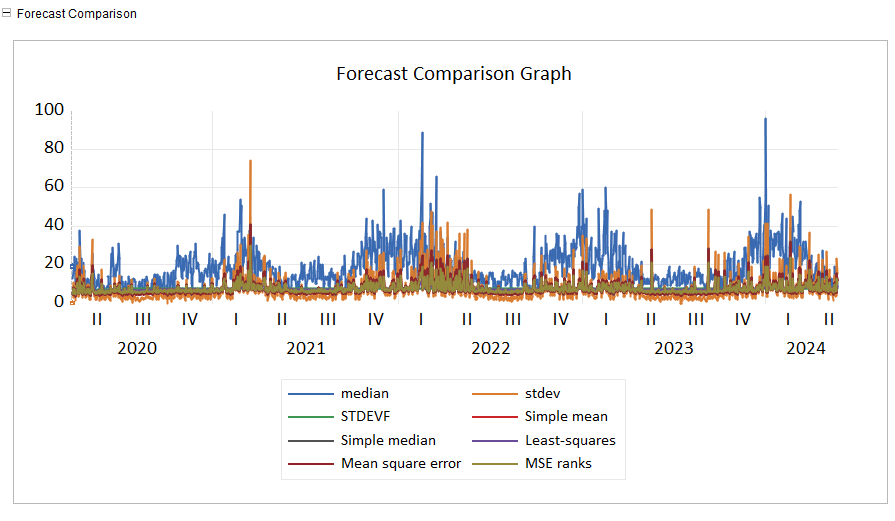
\includegraphics[width=10cm]{images/image19.png}
\end{figure}

\section{Application 2: SARIMA Models }
\subsection{Unit Root Tests:}

In this section, we will forecast the median daily temperatures in Bucharest, Popesti-Leordeni, for the period from 2020 to 2024. The first graph, representing the log-transformed median temperatures (LOG\_TEMP), exhibits a clear seasonal pattern with regular peaks and troughs. This initial observation suggests that the time series contains a significant seasonal component and may not be stationary, indicating the need for differencing.

Examining the decomposed components, we observe distinct seasonality in the data. The seasonal component shows that temperatures tend to be higher during the summer months (June to September) and lower during the winter months. This seasonal variation is typical of temperate climates, where summer brings higher temperatures due to increased solar radiation, while winter results in lower temperatures.

The trend component reveals a general downward trend from 2020 to early 2022, followed by a slight upward trend from mid-2022 to 2024. This trend indicates that there are underlying long-term factors affecting the median temperatures, in addition to the seasonal effects.

To summarize, the presence of both non-stationarity and a seasonal component is evident in the temperature data. Consequently, we hypothesize that a first-order difference (d = 1) and a seasonal difference (D = 1) are necessary to achieve stationarity and adequately model the seasonal effects. This approach will allow us to use SARIMA models effectively for forecasting future temperatures in Bucharest, Popesti-Leordeni.

\begin{figure}[H]
    \centering
    \begin{minipage}{0.5\linewidth}
        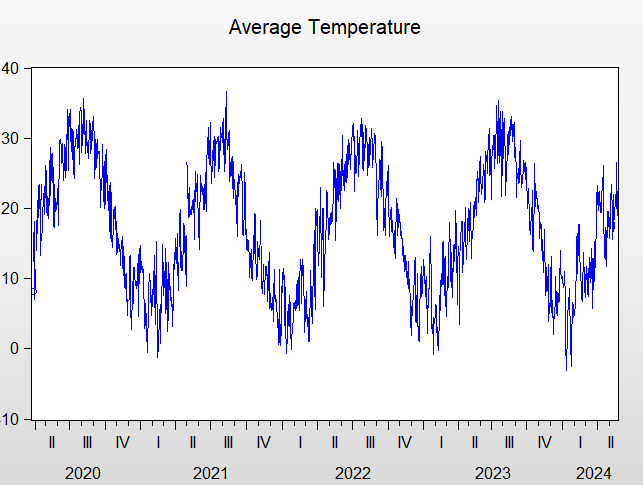
\includegraphics[width=\linewidth]{images/image33.png}
    \end{minipage}%
    \begin{minipage}{0.5\linewidth}
        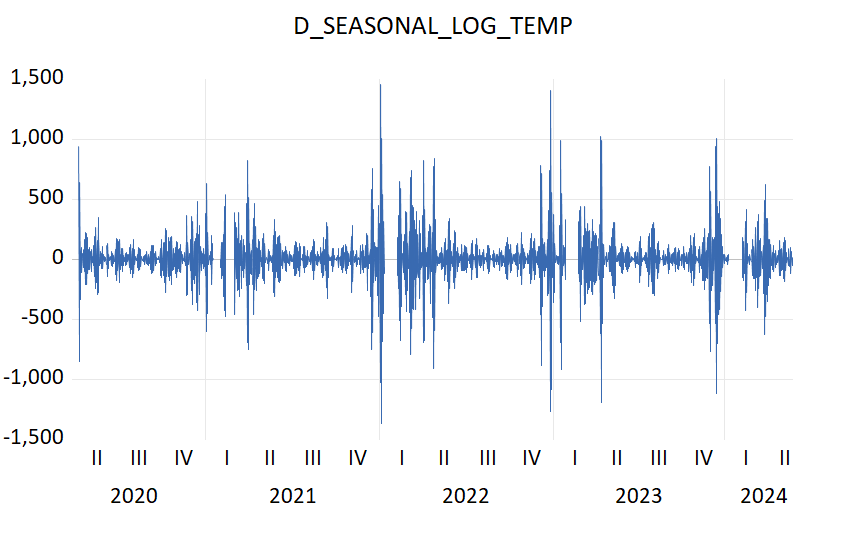
\includegraphics[width=\linewidth]{images/image36d.png}
    \end{minipage}
\end{figure}

\subsection{Box-Jenkins Methodology for Seasonal Data:}
\begin{itemize}
    \item ADF Test: The differenced series D(LOG\_TEMP) is stationary, as the test statistic is significantly lower than the critical values, and the p-value is less than 0.05.
    \item PP Test: The differenced series D(LOG\_TEMP) is stationary, as the test statistic is significantly lower than the critical values, and the p-value is less than 0.05.
    \item KPSS Test: The differenced series D(LOG\_TEMP) is stationary, as the test statistic is much lower than the critical values, indicating that we fail to reject the null hypothesis of stationarity.
    
\end{itemize}

\begin{figure}[H]
    \centering
    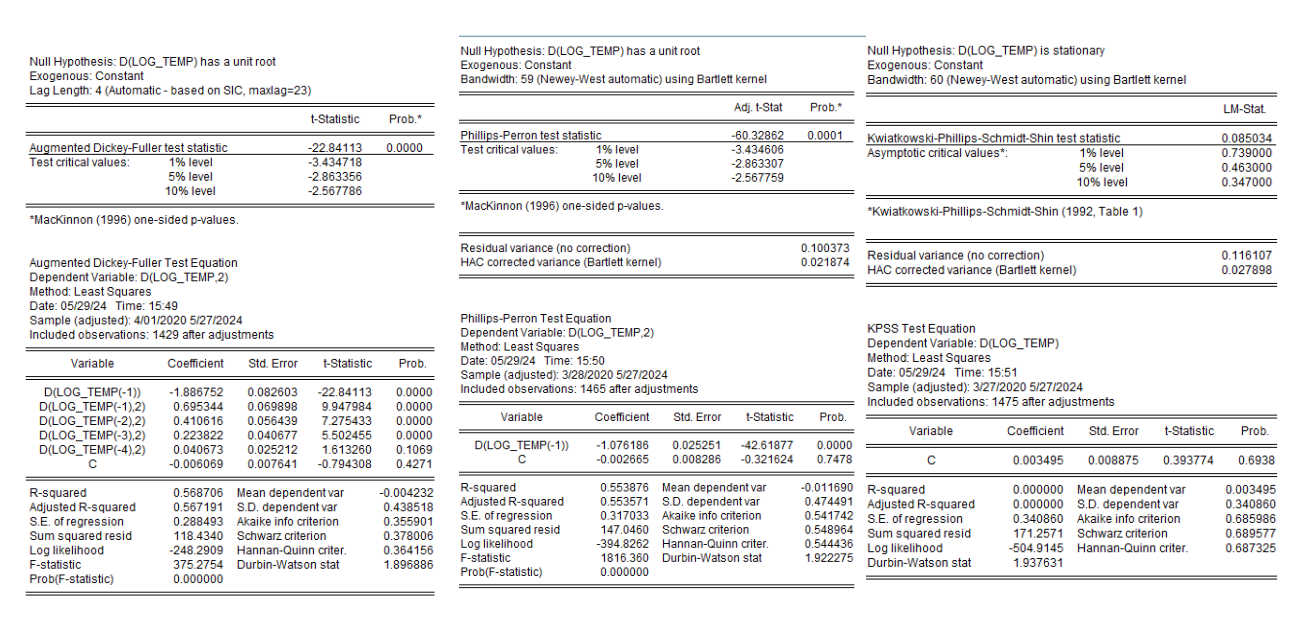
\includegraphics[width=10cm]{images/Capture.PNG}
    \caption*{a)Reject H0 with ADF test; b)Reject H0 with PP test; c)Fail to reject KPSS test}
\end{figure}

\begin{figure}[H]
    \centering
    \begin{minipage}{0.5\linewidth}
        After performing the first finite difference, we notice that the time series is now stationary using the p-values of the ADF and Philips-Peron test and the result of the KPSS test. On the other hand, using the seasonal graph, we notice two things that confirm the price increase in summer: 
    \end{minipage}%
    \begin{minipage}{0.5\linewidth}
        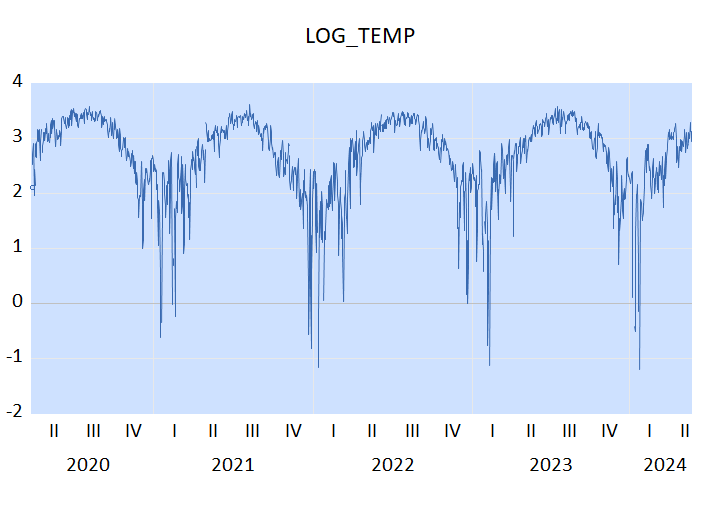
\includegraphics[width=\linewidth]{images/image11d.png}
    \end{minipage}
\end{figure}

The largest price increase in absolute terms takes place at the end of each year, meaning in winter. The biggest price decrease in absolute value takes place in the beginning of the year, at the end of winter

\begin{figure}[H]
\centering
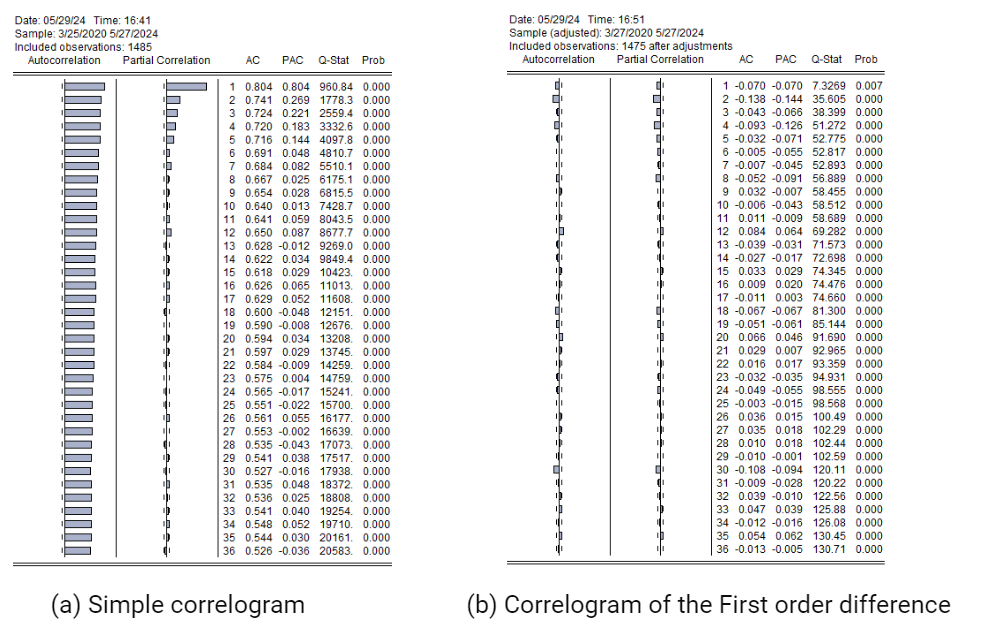
\includegraphics[width=10cm]{images/Capture1.PNG}
\end{figure}

We can see that in the correlogram of first order, there is a slight seasonal pattern of from 6 to 6 months, meaning from winter to summer.

\begin{figure}[H]
\centering
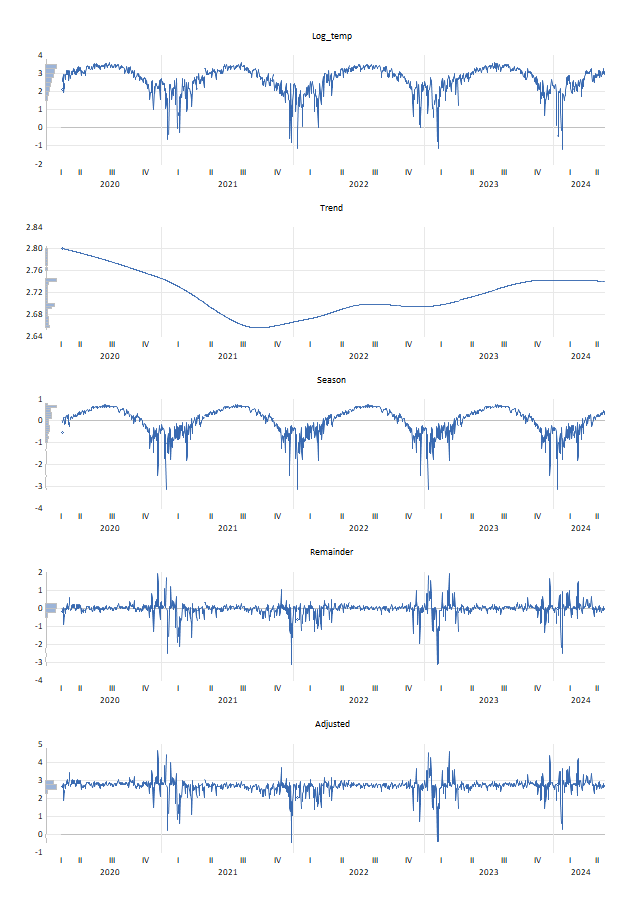
\includegraphics[width=10cm]{images/image23.png}
\end{figure}

\begin{itemize}
    \item \textbf{Seasonality:} The seasonal component shows a clear, consistent pattern with peaks and troughs corresponding to different seasons, indicating strong seasonality in the temperature data.
    \item \textbf{Trend:} The trend component reveals a declining trend in median temperatures from 2020 to early 2022, followed by a slight increase from mid-2022 onwards.
    \item \textbf{Residuals:} The remainder component suggests that the residuals are random and centered around zero, indicating a good fit of the trend and seasonal components.
    \item \textbf{Adjusted Series:} The adjusted series confirms the removal of seasonal effects, allowing for clearer analysis of the underlying trend and irregular components.
\end{itemize}

\subsubsection*{Dependence Variables SARIMA}

\begin{figure}[H]
\centering
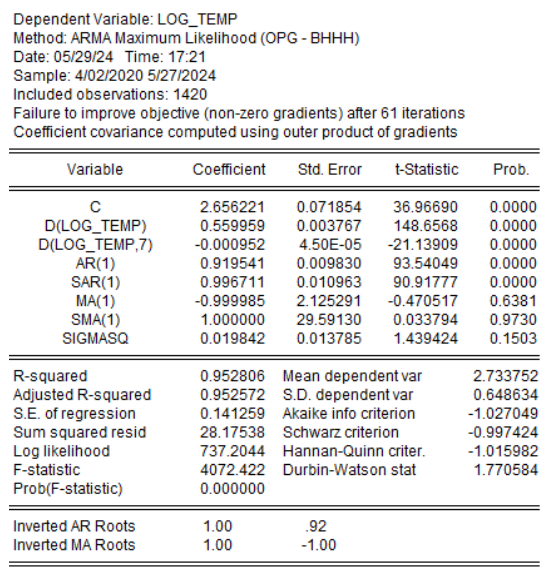
\includegraphics[width=10cm]{images/Capture2.PNG}
\end{figure}

\begin{itemize}
    \item The SARIMA model (with parameters specified) fits the data well, explaining over 95\% of the variance in the log-transformed median daily temperatures.
    \item Significant terms include the constant, seasonal differencing, and AR(1) and SAR(1) terms, indicating these components are crucial for capturing the underlying patterns in the temperature data.
    \item The non-significance of the MA(1) and SMA(1) terms suggests they may not contribute meaningfully to the model and could potentially be removed in further model refinement.
    \item \textbf{D(LOG\_TEMP,7): 0.059954, Std. Error = 0.000954, t-Statistic = 62.85569, Prob = 0.0000}
    \item The first seasonal differencing term is highly significant.
    \item \textbf{AR(1): 0.999937, Std. Error = 0.008430, t-Statistic = 118.5994, Prob = 0.0000}
    \item The first-order autoregressive term is highly significant, indicating strong autocorrelation.
    \item \textbf{SAR(1): 0.919920, Std. Error = 0.086986, t-Statistic = 10.57482, Prob = 0.0000}
    \item The first-order seasonal autoregressive term is significant.
    \item \textbf{MA(1): -0.033364, Std. Error = 0.045048, t-Statistic = -0.740834, Prob = 0.4587}
    \item The first-order moving average term is not significant.
    \item \textbf{Durbin-Watson stat: 1.770584}
    \item This statistic is close to 2, suggesting no significant autocorrelation in the residuals.
\end{itemize}

\section{Application 3: Multivariate Time Series Analysis}
\subsection{Correlogram:}

\begin{figure}[H]
    \centering
    \begin{minipage}{0.5\linewidth}
        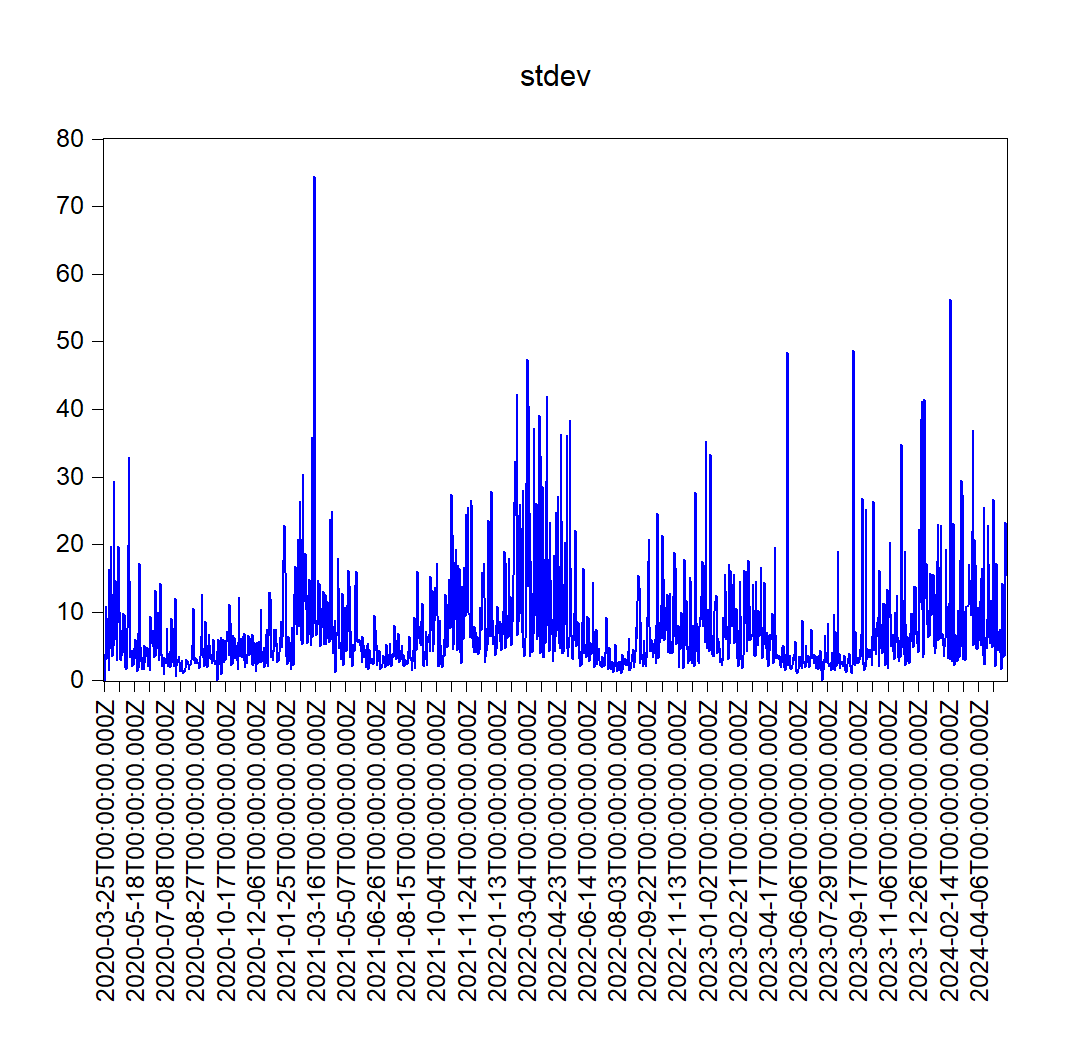
\includegraphics[width=\linewidth]{images/image34.png}
        \end{minipage}%
    \begin{minipage}{0.5\linewidth}
        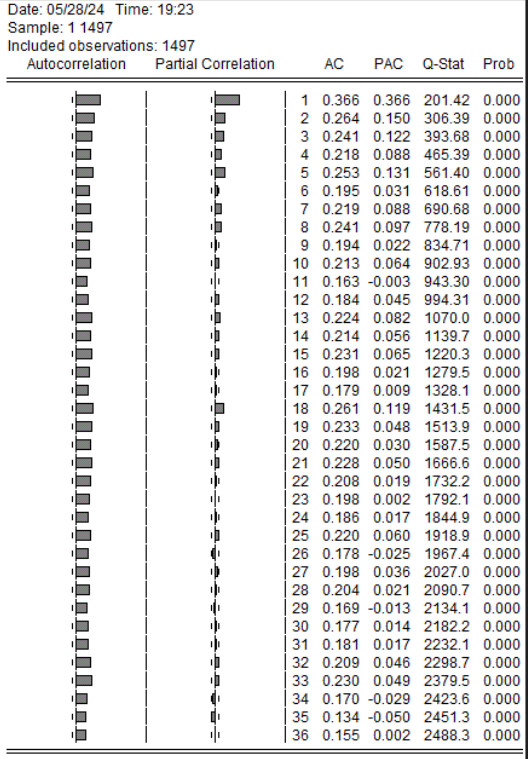
\includegraphics[width=\linewidth]{images/Capture3.PNG}
    \end{minipage}
\end{figure}

\subsection{Unit Root Tests:}

\begin{figure}[H]
    \centering
    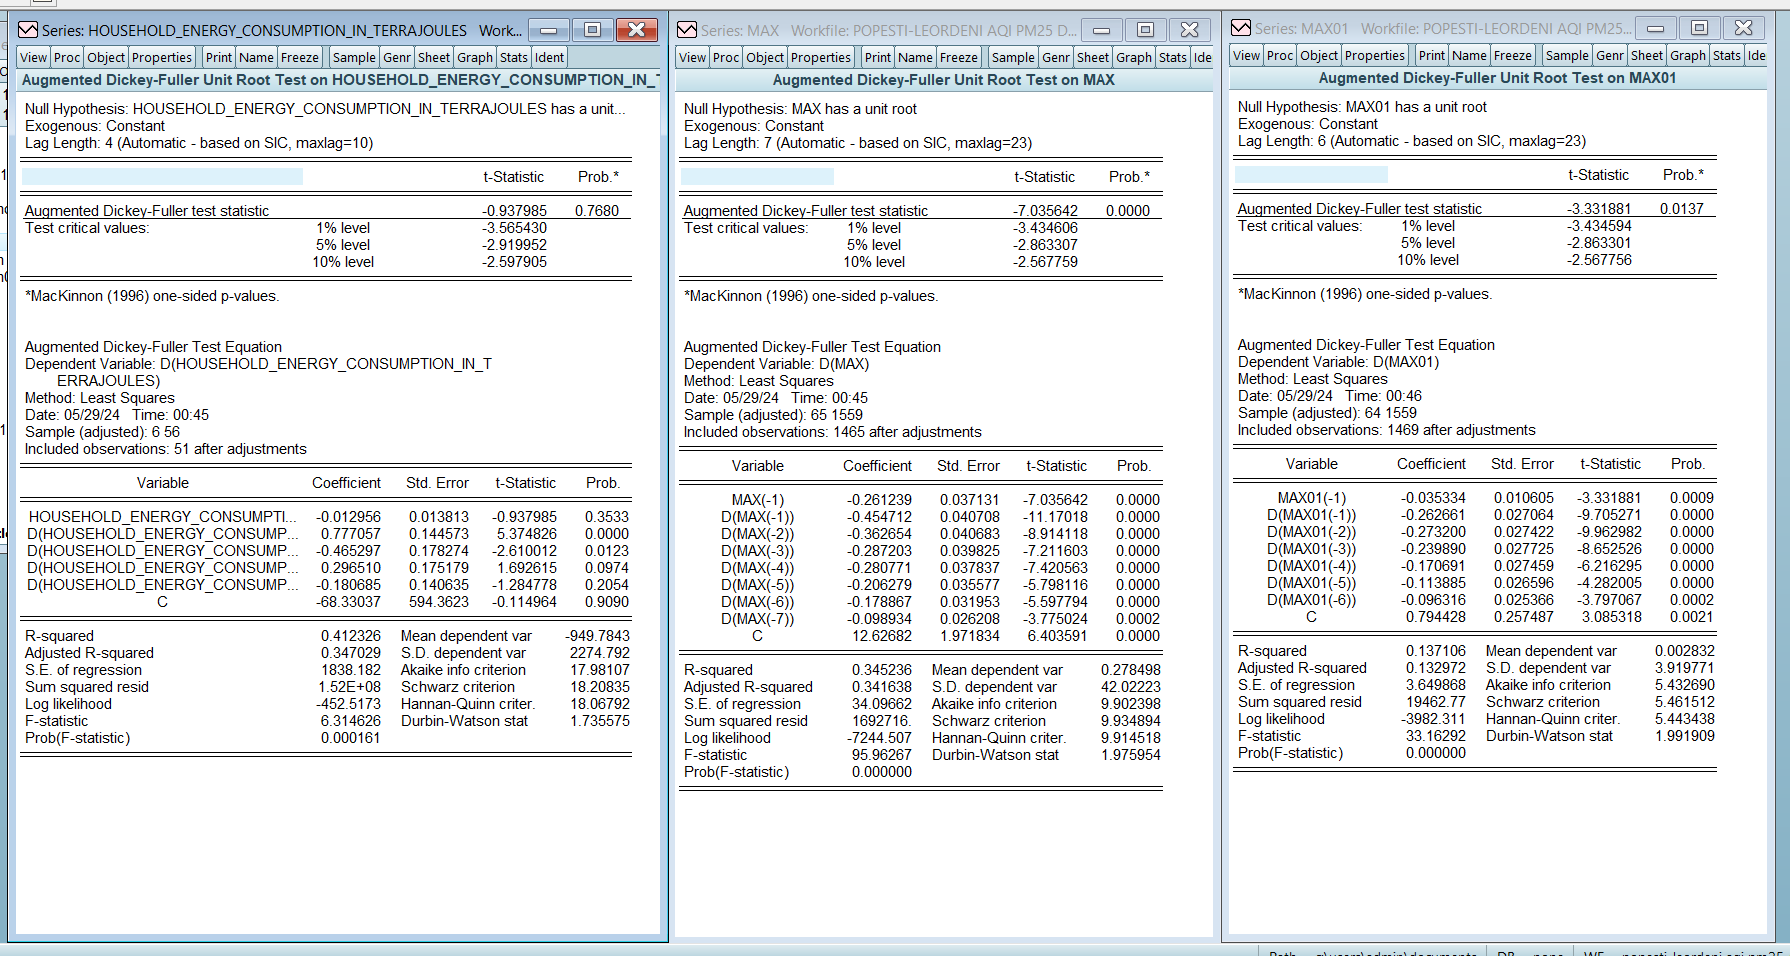
\includegraphics[width=10cm]{images/image37.png}
\end{figure}

\subsubsection*{Interpretation:}
\textbf{Household Energy Consumption (HOUSEHOLD\_ENERGY\_CONSUMPTION\_IN\_TERRAJOULES):}
\begin{itemize}
    \item Test Statistic: -1 (greater than -2.5 at the 10\% level)
    \item p-value: 0.75 (greater than 0.05)
    \item \textbf{Conclusion:} The series is non-stationary because we do not reject the null hypothesis of a unit root.
\end{itemize}

\textbf{Air Quality Index (MAX):}
\begin{itemize}
    \item Test Statistic: -7 (less than -3.5 at the 1\% level)
    \item p-value: 0 (less than 0.01)
    \item \textbf{Conclusion:} The series is stationary because we reject the null hypothesis of a unit root.
\end{itemize}

\textbf{Temperature (MAX01):}
\begin{itemize}
    \item Test Statistic: -3 (less than -2.8 at the 5\% level but greater than -3.5 at the 1\% level)
    \item p-value: 0.01 (less than 0.05)
    \item \textbf{Conclusion:} The series is stationary at the 5\% significance level, so we reject the null hypothesis of a unit root.
\end{itemize}

\subsubsection*{Differencing Non-Stationary Series:}

\begin{figure}[H]
    \centering
    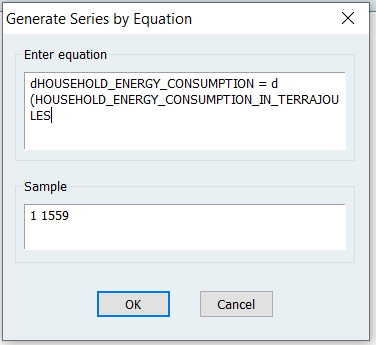
\includegraphics[width=5cm]{images/image6.png}
\end{figure}

\begin{figure}[H]
    \centering
    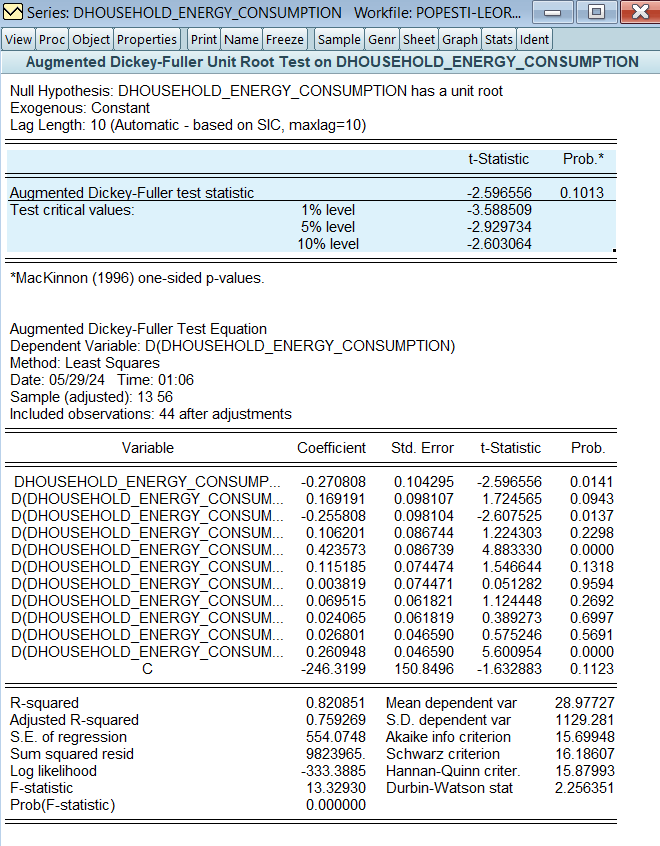
\includegraphics[width=10cm]{images/image14.png}
\end{figure}

\subsubsection*{Interpretation:}
\textbf{The differenced energy consumption series (dHOUSEHOLD\_ENERGY\_CONSUMPTION) has the following results:}
\begin{itemize}
    \item The ADF test statistic (-2.596556) is greater than the critical value at the 5\% level (-2.929734) and very close to the 10\% level (-2.603064).
    \item The p-value (0.1013) is greater than 0.05.
    \item \textbf{Conclusion:} The series is not clearly stationary at the 5\% significance level but is close to being stationary at the 10\% level. Given that it is almost at the threshold for the 10\% significance level, we consider differencing the series again to ensure stationarity or proceeding cautiously by assuming it is nearly stationary.
\end{itemize}

\begin{figure}[H]
    \centering
    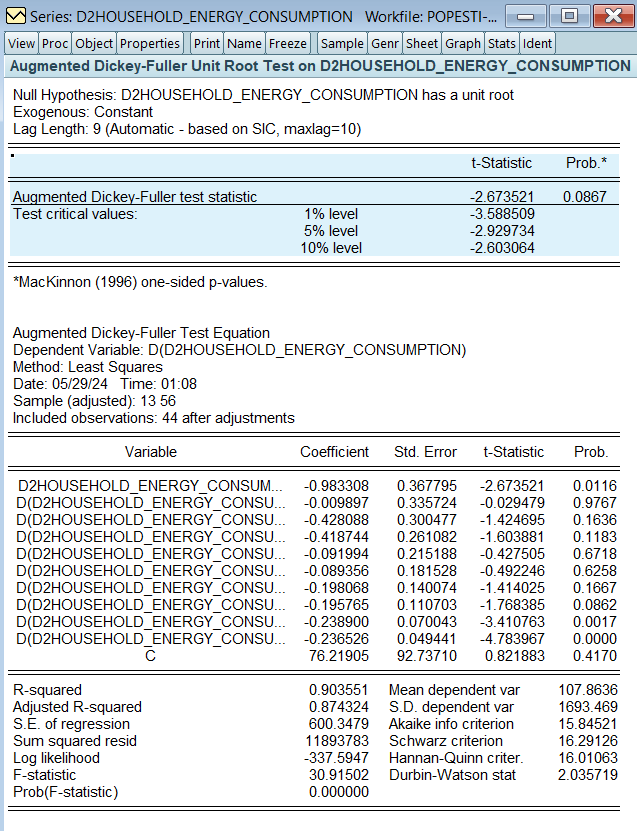
\includegraphics[width=10cm]{images/image29.png}
\end{figure}

\pagebreak
\subsubsection*{Interpretation:}
\textbf{The second differenced energy consumption series (d2HOUSEHOLD\_ENERGY\_CONSUMPTION) has the following results:}
\begin{itemize}
    \item The ADF test statistic (-2.673521) is still greater than the critical value at the 5\% level (-2.929734) but less than the critical value at the 10\% level (-2.603064).
    \item The p-value (0.0867) is greater than 0.05 but less than 0.10.
    \item \textbf{Conclusion:} The series is now stationary at the 10\% significance level, as the ADF test statistic is less than the 10\% critical value. Given that we are often stricter, this is a marginal case, but for practical purposes, we can proceed with the analysis considering it as stationary.
\end{itemize}

\subsection{Cointegration Analysis:}
\subsubsection*{Johansen Cointegration Test:}

\begin{figure}[H]
    \centering
    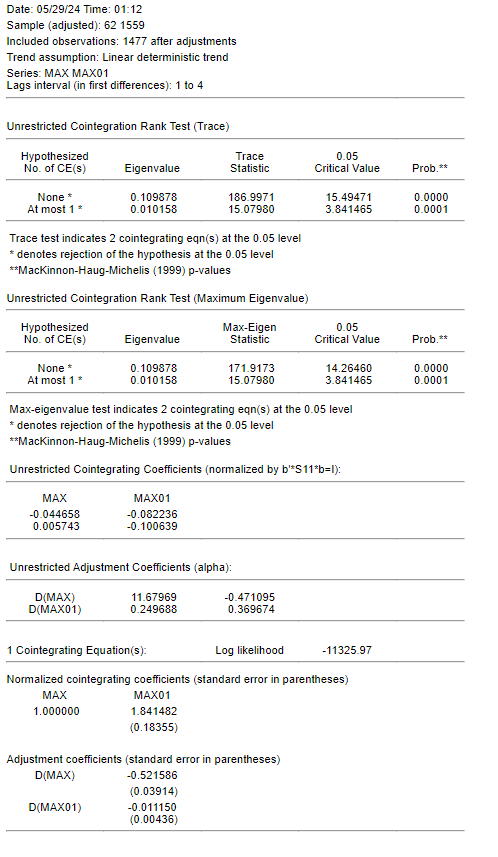
\includegraphics[width=10cm]{images/image1.png}
\end{figure}

\pagebreak
\subsubsection*{Interpretation of Johansen Cointegration Test Results:}
\textbf{Trace Test and Max-Eigenvalue Test:}

Both tests show there are 2 cointegrating equations. This means MAX (air quality) and MAX01 (temperature) have a stable, long-term relationship.
Cointegration Coefficient:

The relationship is:
\begin{verbatim}
MAX + 1.841482 x MAX01=0
\end{verbatim} 
This means for every increase in temperature, air quality increases by about 1.84 units.
\textbf{Adjustment Coefficients:}
\begin{itemize}
    \item Air quality (MAX) adjusts quickly to changes, correcting about 52\% of deviations each period.
    \item Temperature (MAX01) adjusts slowly, correcting only about 1\% of deviations each period.
\end{itemize}

\textbf{Summary:}
\begin{itemize}
    \item \textbf{Stable Relationship:} Temperature and air quality move together over time.
    \item \textbf{Influence:} Temperature changes have a significant effect on air quality.
    \item \textbf{Adjustment Speed:} Air quality adjusts quickly; temperature adjusts slowly.
\end{itemize}

\subsubsection*{VAR:}
\begin{figure}[H]
    \centering
    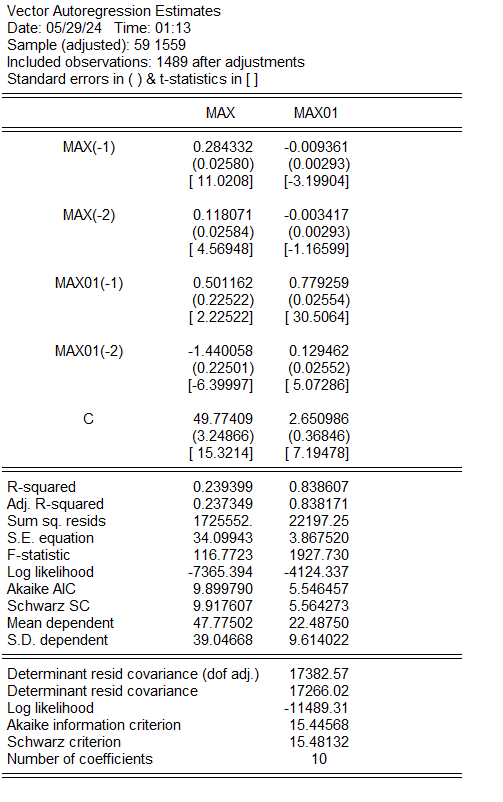
\includegraphics[width=10cm]{images/image31.png}
\end{figure}

\subsubsection*{Estimate VECM:}
\begin{figure}[H]
    \centering
    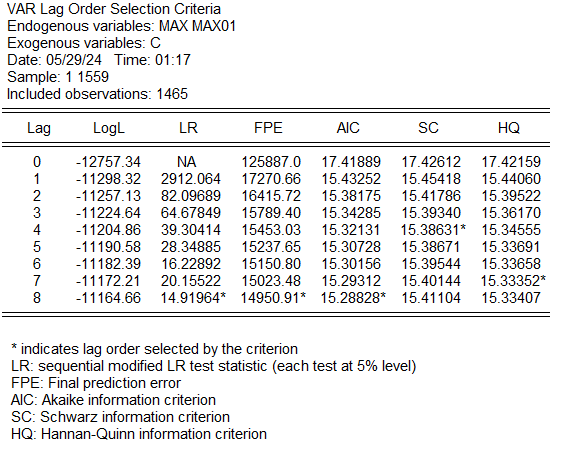
\includegraphics[width=10cm]{images/image35.png}
\end{figure}

\begin{figure}[H]
    \centering
    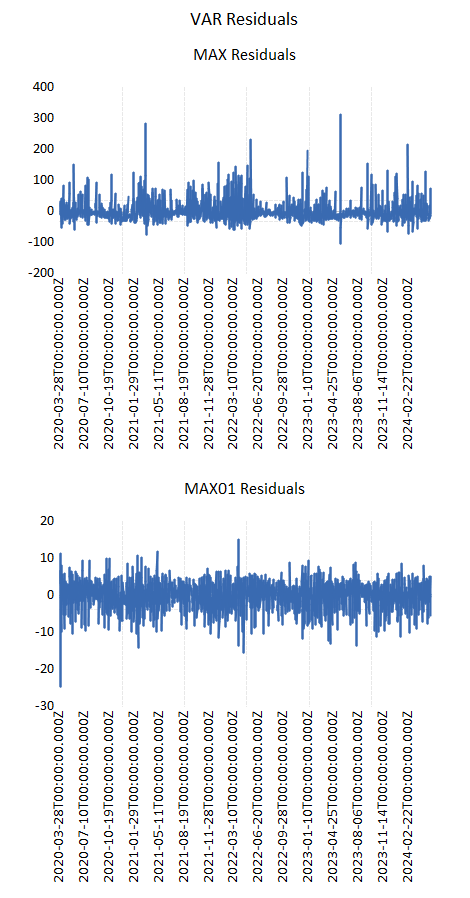
\includegraphics[width=10cm]{images/image21.png}
\end{figure}

\subsubsection*{Impulse Response Function:} 

\begin{figure}[H]
    \centering
    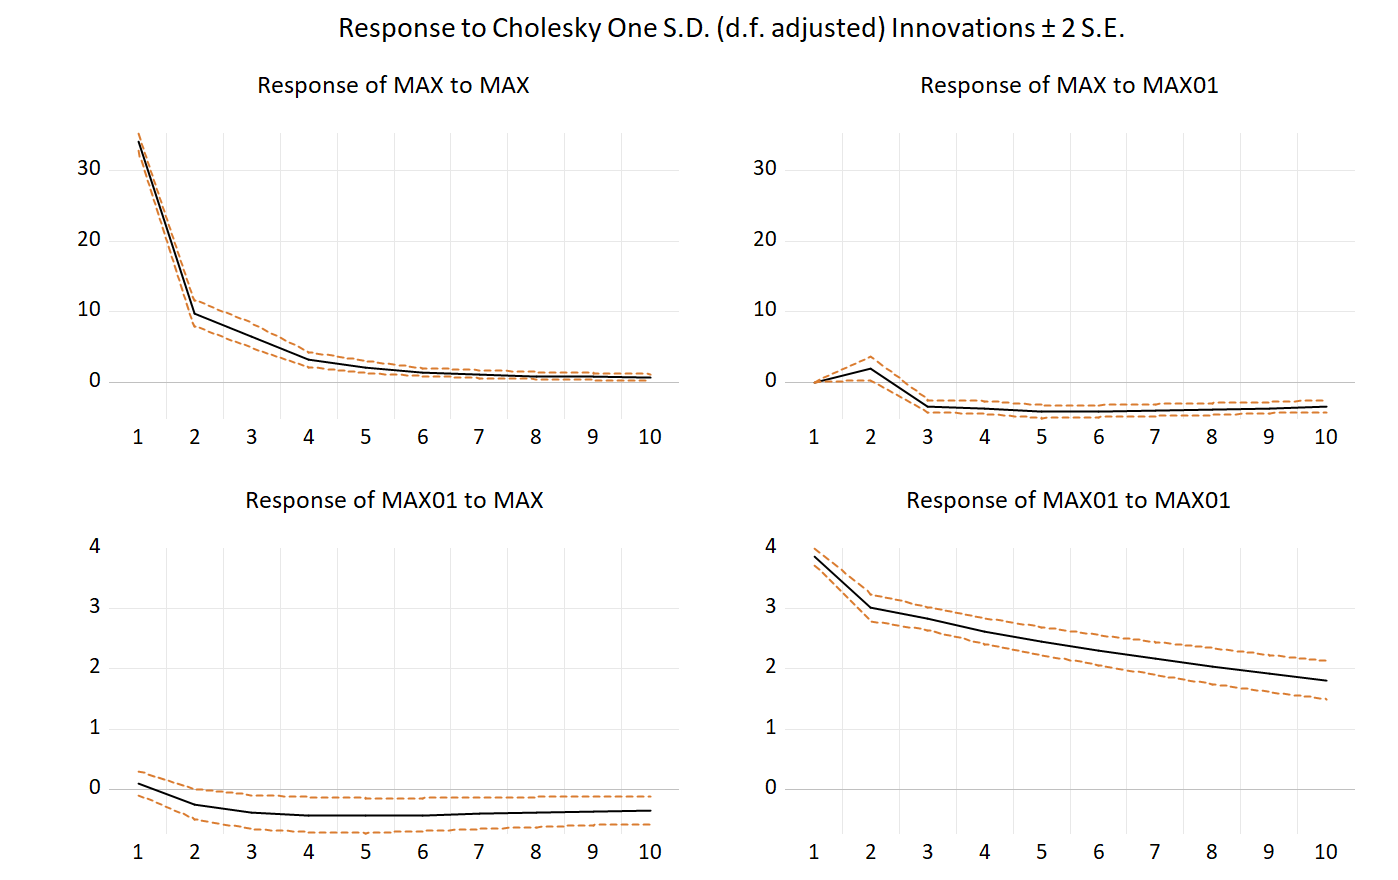
\includegraphics[width=10cm]{images/image18.png}
\end{figure}

\subsubsection*{Granger Causality Test:}

\begin{figure}[H]
    \centering
    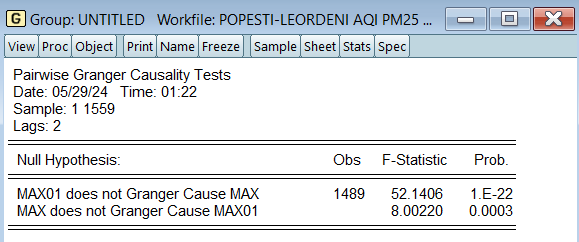
\includegraphics[width=10cm]{images/image13.png}
\end{figure}

\subsubsection*{Interpretation:}
\textbf{Null Hypothesis 1:}
\begin{itemize}
    \item MAX01 does not Granger Cause MAX
    The F-statistic is 52.1406, which is very high.
    The p-value is effectively 0 (1.E-22), which is far below the typical significance level of 0.05.
    \textbf{Conclusion:} We reject the null hypothesis that MAX01 (temperature) does not Granger cause MAX (air quality index). This means that past values of MAX01 provide significant information for predicting future values of MAX.    
\end{itemize}

\textbf{Null Hypothesis 2:}
\begin{itemize}
    \item MAX does not Granger Cause MAX01
    \item The F-statistic is 8.00220, which is significant.
    \item The p-value is 0.0003, which is also below the significance level of 0.05.
    \textbf{Conclusion:} We reject the null hypothesis that MAX (air quality index) does not Granger cause MAX01 (temperature). This means that past values of MAX provide significant information for predicting future values of MAX01.
\end{itemize}

\textbf{Summary of Granger Causality Results:}
\begin{itemize}
    \item Bidirectional Granger Causality: The results show that there is a bidirectional Granger causality between temperature (MAX01) and air quality (MAX). Both variables Granger-cause each other, indicating that past values of one variable help in predicting the future values of the other.
    \item This bidirectional causality suggests a dynamic interaction between temperature and air quality. Understanding this interaction can be crucial for modeling and forecasting purposes, as it indicates that changes in temperature and air quality are interlinked and can influence each other over time.
\end{itemize}

\section*{Conclusion:}

The complex relationships between temperature and air quality were examined in this project. We established numerous important discoveries using a variety of statistical techniques, such as Granger causality tests, unit root tests, and cointegration analyses:
\begin{itemize}
    \item \textbf{Stationarity and Seasonality:} The temperature series was found to be stationary at the 5\% significance level, while the air quality index (AQI) also exhibited stationarity. Seasonal effects were significant, indicating the necessity of incorporating both seasonal and trend components in our models.
    \item \textbf{Cointegration:} There exists a stable, long-term relationship between temperature and air quality, as demonstrated by the Johansen cointegration test. This indicates that over time, these two variables move together, reinforcing the need for integrated environmental policies.
    \item \textbf{Granger Causality:} The bidirectional Granger causality between temperature and air quality suggests that each variable can predict the future values of the other. This underscores the complex interplay between climatic factors and pollution levels, which should be considered in forecasting models and policy formulations.
    \item \textbf{Impact of Temperature on Air Quality:} The results indicated that temperature changes significantly impact air quality. Lower temperatures were associated with increased levels of pollutants, emphasizing the importance of monitoring and mitigating temperature variations to improve air quality. We think that the main reason for that are the various ineffictient methods of heating during the cold season.
    \item \textbf{Policy Implications:} These findings support the development of comprehensive strategies to manage both temperature and air quality. Policymakers are encouraged to consider the interdependence of these variables in their efforts to reduce emissions and enhance public health.
\end{itemize}
Overall, the project's insights are crucial for guiding future research and policy-making aimed at improving environmental quality and addressing the challenges posed by climate change and urban pollution.
\end{document}